\begin{flushright} {\tiny {\color{gray} benchmark\_annulus\_converction\_benchmark1.tex}} \end{flushright}
%~~~~~~~~~~~~~~~~~~~~~~~~~~~~~~~~~~~~~~~~~~~~~~~~~~~~~~~~~~~~~~~~~~~~~~~~~~~~~~~~~~~~~~~~~~~~~~~~~~

We wish to solve the Stokes equation in an annulus of inner radius $R_1$
and outer radius $R_2$ with the following boundary conditions:
\begin{itemize}
\item Inner boundary: $\upnu_r(R_1,\theta)=0$ 
\item Outer boundary: $\upnu_r(R_2,\theta)=0$ 
\end{itemize}
We then postulate
\[
\upnu_\theta(r,\theta)= f(r) \cos(k\theta)
\]
Note that in the case $k=0$, we recover a constant velocity on the inner and outer boundaries.

The divergence of an incompressible vector field in polar coordinates is
\[
\frac{1}{r} \frac{\partial (r\upnu_r)}{\partial r} + \frac{1}{r} \frac{\partial \upnu_\theta}{\partial \theta} =0
\]
or, 
\[
\frac{\partial (r\upnu_r)}{\partial r} + \frac{\partial \upnu_\theta}{\partial \theta} =0
\]
i.e.,
\[
\frac{\partial (r\upnu_r)}{\partial r} = - \frac{\partial \upnu_\theta}{\partial \theta} = k f(r) \sin(k\theta) 
\]
so 
\[
r\upnu_r(r,\theta) = k \left[ \int f(r) dr \right] \sin(k\theta) 
\]
and finally 
\[
\upnu_r(r,\theta) = k g(r) \sin(k\theta)  
\]
with 
\begin{eqnarray}
g(r)  &=& \frac{1}{r} \int f(r) dr \\
g'(r) &=& -\frac{1}{r^2} \int f(r) dr + \frac{1}{r} f = - \frac{1}{r} g + \frac{1}{r} f = \frac{1}{r}(f-g) 
\end{eqnarray}


The boundary conditions lead to
\[
\upnu_r(r=R_1,\theta) = 
k (\frac{A}{2}R_1 + \frac{B}{R_1} \ln R_1 + \frac{C}{R_1}) \sin(k\theta)  = 0
\]
\[
\upnu_r(r=R_2,\theta) = 
k (\frac{A}{2}R_2 + \frac{B}{R_2} \ln R_2 + \frac{C}{R_2}) \sin(k\theta)  = 0
\]
This has to be valid $\forall \theta$, so 
%\[
%\frac{A}{2}R_1^2 + B \ln R_1 - 1 =0 
%\]
%\[
%\frac{A}{2}R_2^2 + B \ln R_2 - 1 = 0
%\]
%or, 
\[
\frac{A}{2}R_1^2 + B \ln R_1 =-C
\quad\quad {\rm and} \quad\quad
\frac{A}{2}R_2^2 + B \ln R_2 =-C
\]
leading to 
\[
\frac{A}{2}+ \frac{B}{R_1^2} \ln R_1 =-\frac{C}{R_1^2}
\quad\quad {\rm and} \quad\quad
\frac{A}{2}+ \frac{B}{R_2^2} \ln R_2 =-\frac{C}{R_2^2}
\]
and finally 
\[
B = -C \frac{R_2^2-R_1^2}{R_2^2 \ln R_1 - R_1^2 \ln R_2}
\]
Likewise
\[
\frac{A}{2}R_1^2 + B \ln R_1 = -C
\quad\quad {\rm and} \quad\quad
\frac{A}{2}R_2^2 + B \ln R_2 = -C
\]
yields
\[
\frac{A}{2 \ln R_1}R_1^2 + B  = -\frac{C}{\ln R_1}
\quad\quad {\rm and} \quad\quad
\frac{A}{2 \ln R_2}R_2^2 + B  = -\frac{C}{\ln R_2}
\]
or, 
\[
\frac{A}{2 \ln R_1}R_1^2 - \frac{A}{2 \ln R_2}R_2^2  =  -C (\frac{1}{\ln R_1} - \frac{1}{\ln R_2})
\]
\[
A (\frac{R_1^2}{2 \ln R_1} - \frac{R_2^2}{2 \ln R_2})  =  -C (\frac{1}{\ln R_1} - \frac{1}{\ln R_2})
\]
\[
A (\frac{R_1^2 \ln R_2 }{2 } - \frac{R_2^2 \ln R_1 }{2} )  = -C( \ln R_2 - \ln R_1)
\]
finally
\[
A = -C\frac{2(\ln R_2 - \ln R_1)} { R_1^2 \ln R_2  - R_2^2 \ln R_1}    
= -C\frac{2(\ln R_1 - \ln R_2)} { R_2^2 \ln R_1  - R_1^2 \ln R_2}    
\]


We set ${\vec g}=-g_r {\vec e}_r$.
Stokes equation in Polar coordinates (p284 of Schubert, Turcotte and Olson book):
\begin{itemize}
\item 
$r$-component:
\[
\eta \left[ \nabla^2 \upnu_r - \frac{\upnu_r}{r^2} - \frac{2}{r^2} \frac{\partial \upnu_\theta}{\partial \theta}  \right]
+
\frac{\eta}{3} \frac{\partial}{\partial r} \left[ \frac{1}{r}\frac{\partial (r \upnu_r)}{\partial r} 
+ \frac{1}{r} \frac{\partial \upnu_\theta}{\partial \theta}  \right]
-\frac{\partial p}{\partial r} - \rho g_r = 0
\]
The second term between brackets in the divergence of the velocity field so it is equal to zero in our case. We end up with 
\[
\eta \left[ \nabla^2 \upnu_r - \frac{\upnu_r}{r^2} - \frac{2}{r^2} \frac{\partial u_\theta}{\partial \theta}  \right]
-\frac{\partial p}{\partial r} - \rho g_r = 0
\]
\item 
$\theta$-component:
\[
\eta \left[ \nabla^2 \upnu_\theta +\frac{2}{r^2} \frac{\partial \upnu_r}{\partial \theta} - \frac{\upnu_\theta}{r^2} \right]
+
\frac{\eta}{3} \frac{1}{r} \frac{\partial }{\partial \theta} 
\left[
\frac{1}{r}\frac{\partial (r \upnu_r)}{\partial r} + \frac{1}{r} \frac{\partial \upnu_\theta}{\partial \theta} 
\right]
- \frac{1}{r} \frac{\partial p}{\partial \theta}  = 0
\]
The second term between brackets in the divergence of the velocity field so it is equal to zero in our case. We end up with 
\[
\eta \left[ \nabla^2 \upnu_\theta +\frac{2}{r^2} \frac{\partial \upnu_r}{\partial \theta} - \frac{\upnu_\theta}{r^2} \right]
- \frac{1}{r}\frac{\partial p}{\partial \theta} = 0
\]
\end{itemize}
In both equations, $\nabla^2$ represents the Laplacian of a scalar quantity:
\[
\nabla^2 = \frac{\partial^2}{\partial r^2} + \frac{1}{r} \frac{\partial }{\partial r} + \frac{1}{r^2} \frac{\partial^2 }{\partial \theta^2}
\]
We can then write the two momentum equations for an incompressible Stokes flow in polar coordinates:
\[
\eta \left[ 
\frac{\partial^2 \upnu_r}{\partial r^2} + \frac{1}{r} \frac{\partial \upnu_r}{\partial r} 
+ \frac{1}{r^2} \frac{\partial^2 \upnu_r}{\partial \theta^2}
- \frac{\upnu_r}{r^2} - \frac{2}{r^2} \frac{\partial \upnu_\theta}{\partial \theta}  \right]
-\frac{\partial p}{\partial r} - \rho g_r = 0
\]
\[
\eta \left[ 
\frac{\partial^2 \upnu_\theta}{\partial r^2} + \frac{1}{r} \frac{\partial \upnu_\theta}{\partial r} 
+ \frac{1}{r^2} \frac{\partial^2 \upnu_\theta}{\partial \theta^2}
+\frac{2}{r^2} \frac{\partial \upnu_r}{\partial \theta} - \frac{\upnu_\theta}{r^2} \right]
- \frac{1}{r}\frac{\partial p}{\partial \theta}  = 0
\]
We can further choose $\eta=1$, so that 
\begin{equation}
\frac{\partial^2 \upnu_r}{\partial r^2} + \frac{1}{r} \frac{\partial \upnu_r}{\partial r} 
+ \frac{1}{r^2} \frac{\partial^2 \upnu_r}{\partial \theta^2}
- \frac{\upnu_r}{r^2} - \frac{2}{r^2} \frac{\partial \upnu_\theta}{\partial \theta} 
-\frac{\partial p}{\partial r} - \rho g_r = 0
\label{eq1}
\end{equation}
\begin{equation}
\frac{\partial^2 \upnu_\theta}{\partial r^2} + \frac{1}{r} \frac{\partial \upnu_\theta}{\partial r} 
+ \frac{1}{r^2} \frac{\partial^2 \upnu_\theta}{\partial \theta^2}
+\frac{2}{r^2} \frac{\partial \upnu_r}{\partial \theta} - \frac{\upnu_\theta}{r^2} 
-\frac{1}{r}\frac{\partial p}{\partial \theta} = 0
\label{eq2}
\end{equation}

Let us define $f(r)= Ar+B/r$. We then have 
\begin{eqnarray}
 \frac{\partial^2 f}{\partial r^2} + \frac{1}{r} \frac{\partial f}{\partial r} - \frac{f}{r^2} 
&=& A \left( \frac{\partial^2 r}{\partial r^2} + \frac{1}{r} \frac{\partial r}{\partial r} - \frac{1}{r}\right) 
+ B \left(\frac{\partial^2 r^{-1}}{\partial r^2} + \frac{1}{r} \frac{\partial r^{-1}}{\partial r}  - \frac{1}{r^3}\right) =0
%\nn\\
%&=& \frac{A}{r} + B \left( \frac{2}{r^3} - \frac{1}{r^3}  \right) - \frac{A}{r} -  \frac{B}{r^3}  \nn\\
%&=& 0 \nn
\end{eqnarray}
Eq. (\ref{eq2}) simplifies to:
\[
\frac{1}{r^2} \frac{\partial^2 \upnu_\theta}{\partial \theta^2}
+\frac{2}{r^2} \frac{\partial \upnu_r}{\partial \theta} 
-\frac{1}{r}\frac{\partial p}{\partial \theta} = 0
\]
We have 
\[
\frac{1}{r^2} \frac{\partial^2 \upnu_\theta}{\partial \theta^2}
=
-k^2\frac{f(r)}{r^2} \cos (k \theta)  %= -\frac{k^2}{r^2} v_\theta
\quad\quad {\rm and} \quad\quad
\frac{2}{r^2} \frac{\partial \upnu_r}{\partial \theta} 
=
\frac{2k^2}{r^2} g(r)  \cos(k \theta) 
\]
so 
\[
\frac{1}{r}
\frac{\partial p}{\partial \theta} = 
-\frac{k^2}{r^2}f(r) \cos (k \theta) 
+ 
\frac{2k^2}{r^2} g(r)  \cos(k \theta) 
= k^2\left(  \frac{2g(r)-f(r)}{r^2} \right) \cos(k \theta)
\]
and then 
\[
\frac{\partial p}{\partial \theta} = 
 k^2\left(  \frac{2g(r)-f(r)}{r} \right) \cos(k \theta)
\]
This can be integrated with respect to $\theta$:
\[
p(r,\theta)= k\left(  \frac{2g(r)-f(r)}{r} \right) \sin(k \theta) +  l(r)
= k h(r) \sin(k \theta) + l(r)
\]
where $h(r) = \frac{1}{r}(2g(r)-f(r))$.
We can turn to Eq.(\ref{eq1}). 
\begin{eqnarray}
\rho g_r 
&=& 
 \frac{\partial^2 \upnu_r}{\partial r^2} 
+ \frac{1}{r} \frac{\partial \upnu_r}{\partial r} 
+ \frac{1}{r^2} \frac{\partial^2 \upnu_r}{\partial \theta^2}
- \frac{\upnu_r}{r^2} 
- \frac{2}{r^2} \frac{\partial \upnu_\theta}{\partial \theta} 
-\frac{\partial p}{\partial r}  \nn\\
&=& 
+ k g''(r) \sin (k \theta) 
+ k \frac{g'(r)}{r} \sin (k \theta) 
- k^3 \frac{g(r)}{r^2} \sin(k\theta) 
- k \frac{g(r)}{r^2} \sin(k \theta) 
+ k \frac{2f(r)}{r^2}  \sin(k \theta)
- k h'(r) \sin(k \theta) 
- l'(r) \nn\\
&=& k \sin(k\theta)
\left[ g'' + \frac{g'}{r} - \frac{k^2 g }{r^2} - \frac{g}{r^2} + \frac{2f}{r^2} - h'  \right] - l'(r) \nn\\
&=& k \sin(k\theta)
\left[ g'' + \frac{g'}{r} - \frac{k^2 g }{r^2} - \frac{g}{r^2} + \frac{2f}{r^2} + \frac{1}{r^2} (2g-f) - \frac{1}{r} (2g'-f')   \right] - l'(r) \nn\\
&=& k \sin(k\theta)
\left[ g'' + \frac{g'}{r} ( 1 - 2) - \frac{g}{r^2} (k^2 + 1 -2)  + \frac{f}{r^2}  (2-1)  + \frac{f'}{r}   \right] - l'(r) \nn\\
&=& k \sin(k\theta)
\left[ g'' - \frac{g'}{r}  - \frac{g}{r^2} (k^2 - 1)  + \frac{f}{r^2}   + \frac{f'}{r}   \right] - l'(r) 
\end{eqnarray}

We can further choose $g_r=1$. Note that when $k=0$, we have $\rho = -l'(r) $.
We then choose $l'(r)=-\rho_0$ so that the $k$-dependent term can be seen as a density perturbation:
\[
\rho = k \sin (k \theta) \aleph(r) + \rho_0
\]
with 
\[
\aleph(r) = 
g'' + \frac{g'}{r} ( 1 - \frac{2}{r}) - \frac{g}{r^2} (k^2 + 1 -\frac{4}{r}) + \frac{2f}{r^2}  (1-\frac{1}{r}) + \frac{f'}{r^2}  
\]
and
\begin{eqnarray}
f(r)   &=& Ar +\frac{B}{r}\\
f'(r)  &=& A - \frac{B}{r^2}\\
g(r)   &=& \frac{A}{2}r  +  \frac{B}{r} \ln r - \frac{1}{r}\\
g'(r)  &=& \frac{A}{2}  +  \frac{B}{r^2} (1-\ln r)   + \frac{1}{r^2}\\
g''(r) &=& -\frac{2B}{r^3} (1-\ln r)  - B \frac{1}{r^3}  - \frac{2}{r^3} = - \frac{B}{r^3} (3 - 2 \ln r ) 
\end{eqnarray}
Finally, the pressure is then given by 
\[
p(r,\theta)= k\left(  \frac{2g-f}{r^2} \right) \sin(k \theta) +  l(r)
= k h(r) \sin(k \theta) + \rho_0 g_r r + Constant
\]
We enforce $p(r=R_2,\theta)=0$ so that 
\[
p(r,\theta)= k\left(  \frac{2g-f}{r^2} \right) \sin(k \theta) +  l(r)
= k h(r) \sin(k \theta) + \rho_0 g_r (r-R_2) 
\]

%..........................................
\paragraph{Summary of the previous pages}:
\begin{eqnarray}
\upnu_\theta(r,\theta) &=& f(r) \cos(k\theta) \\
\upnu_r(r,\theta) &=& g(r) k  \sin(k\theta)  \\
p(r,\theta) &=& k h(r) \sin(k \theta) + \rho_0 g_r (r-R_2)  \\
\rho(r,\theta) &=& k \sin (k \theta) \aleph(r) + \rho_0 \\
A &=& \frac{2(\ln R_1 - \ln R_2)} { R_2^2 \ln R_1  - R_1^2 \ln R_2}    \\
B &=& \frac{R_2^2-R_1^2}{R_2^2 \ln R_1 - R_1^2 \ln R_2} \\
f(r)   &=& Ar +\frac{B}{r} \\
f'(r)  &=& A - \frac{B}{r^2} \\
g(r)   &=& \frac{A}{2}r  +  \frac{B}{r} \ln r - \frac{1}{r} \\
g'(r)  &=& \frac{A}{2}  +  \frac{B}{r^2} (1-\ln r)   + \frac{1}{r^2} \\
g''(r) &=&  - \frac{B}{r^3} (3 - 2 \ln r )  \\
h(r)   &=& \frac{1}{r^2}(2g-f) \\
\aleph(r) &=&  -g'' - \frac{g'}{r} ( 1 - \frac{2}{r}) + \frac{g}{r^2} (k^2 + 1 -\frac{4}{r})  - \frac{2f}{r^2}  (1-\frac{1}{r}) - \frac{f'}{r^2}   
\end{eqnarray}

%..........................................
\paragraph{Averagings of fields}:

\begin{itemize}
\item Average $\upnu_r$ velocity
\[
<\upnu_r(r)> =\frac{1}{2\pi}\int_0^{2\pi} \upnu_r(r,\theta) d\theta
=\frac{1}{2\pi}\int_0^{2\pi}  g(r) k \sin(k \theta) d\theta
=\frac{1}{2\pi}g(r) k \int_0^{2\pi}  \sin(k \theta) d\theta = 0
\]
since $k=0,2,4,...$

\item Average $\upnu_\theta$ velocity
\[
<\upnu_\theta(r)>
=\frac{1}{2\pi}\int_0^{2\pi} \upnu_\theta(r,\theta) d\theta
=\frac{1}{2\pi}\int_0^{2\pi} f(r) \cos(k \theta) d\theta
=\frac{1}{2\pi}f(r)\int_0^{2\pi}  \cos(k \theta) d\theta
=0
\]
since $k=0,2,4,...$

\item Root mean square verage $\upnu_r$ velocity
\begin{eqnarray}
<\upnu_r>_{rms}(r) 
&=& \sqrt{\frac{1}{2\pi} \int_0^{2\pi} \upnu_r^2 d\theta }   \nn\\
&=& \sqrt{\frac{1}{2\pi} g(r)^2 k^2\int_0^{2\pi} \sin^2 (k \theta) d\theta }   \nn\\
&=& \sqrt{\frac{1}{2\pi} g(r)^2 k^2\int_0^{2\pi} \frac{1}{2}(1-\cos (2k\theta)  ) d\theta }   \nn\\
&=& \sqrt{\frac{1}{2\pi} g(r)^2 k^2  \left(\pi - \frac{1}{2}  \int_0^{2\pi} \cos (2k\theta)   d\theta \right) }   \nn\\
&=& \sqrt{\frac{1}{2\pi} g(r)^2 k^2  \left(\pi - \frac{1}{4k} \underbrace{ \int_0^{2k\pi} \cos \alpha   d\alpha}_{=0} \right) }   \nn\\
&=& \frac{k|g(r)|}{\sqrt{2}} 
\end{eqnarray}

\item Root mean square verage $\upnu_\theta$ velocity

\begin{eqnarray}
<\upnu_\theta>_{rms}(r) 
&=& \sqrt{\frac{1}{2\pi} \int_0^{2\pi} \upnu_\theta^2 d\theta }   \nn\\
&=& \sqrt{\frac{1}{2\pi} f(r)^2 \int_0^{2\pi} \cos^2(k \theta) d\theta }  \nn\\
&=& \sqrt{\frac{1}{2\pi} f(r)^2 \int_0^{2\pi}  \frac{1}{2}(1 + \cos (2k\theta))   d\theta }  \nn\\
&=& \sqrt{\frac{1}{2\pi} f(r)^2 \left( \pi + \frac{1}{2} \int_0^{2\pi}   \cos (2k\theta) d\theta \right)  }  \nn\\
&=& \sqrt{\frac{1}{2\pi} f(r)^2 \left( \pi + \frac{1}{4k} \underbrace{\int_0^{4k\pi}   \cos \alpha d\alpha}_{0} \right)  }  \nn\\
&=& \frac{|f(r)|}{\sqrt{2}}
\end{eqnarray}

\item Root mean square velocity $\upnu_{rms}$

\begin{eqnarray}
\upnu_{rms}=\sqrt{\frac{1}{V}\int_V (\upnu_r^2+\upnu_\theta^2)dV   }
\end{eqnarray}

The volume of the domain is given by 
\[
V=\pi(R_2^2-R_1^2)
\]
and the sum
\begin{eqnarray}
(\upnu_r^2+\upnu_\theta^2 )dV 
&=& [(g(r) k  \sin(k\theta))^2+    (f(r) \cos (k\theta))^2] rdrd\theta \nn\\
&=& [g(r)^2r dr] [k^2  \sin^2(k\theta) d\theta ]+    [f(r)^2 r dr] [ \cos^2 (k\theta) d\theta] \nn
\end{eqnarray}

If $k=0$, we have  $\upnu_\theta = f(r)$ and $\upnu_r = 0$ so that 
%=\sqrt{\frac{1}{V}\int_V (v_r^2+v_\theta^2)dV   }
%=\sqrt{\frac{1}{V}\int_0^{2\pi} \int_{R_1}^{R_2} f(r)^2 r dr d\theta   }

\begin{eqnarray}
\upnu_{rms}
&=& \sqrt{ \frac{1}{V}  \int_0^{2\pi}  d\theta  \int_{R_1}^{R_2} f(r)^2 r dr  } \nn\\
&=& \sqrt{ \frac{2 \pi}{\pi(R_2^2-R_1^2) }     \int_{R_1}^{R_2} f(r)^2 r dr  } \nn\\
&=& \sqrt{ \frac{2 }{(R_2^2-R_1^2) }    \int_{R_1}^{R_2} \left( Ar + \frac{B}{r} \right)^2 r dr } \nn\\
&=& \sqrt{ \frac{2 }{(R_2^2-R_1^2) }   \int_{R_1}^{R_2} \left( A^2r^3 + 2ABr + \frac{B^2}{r}  \right) dr } \nn\\
&=& \sqrt{ \frac{2 }{(R_2^2-R_1^2) }    \left[ A^2 \frac{r^4}{4} + ABr^2 + B^2 \ln(r)  \right]_{R_1}^{R_2} } \nn\\
&=& \sqrt{ \frac{2 }{(R_2^2-R_1^2) }  [ \frac{A^2}{4}(R_2^4-R_1^4) + AB (R_2^2-R_1^2) + B^2 (\ln R_2 - \ln R_1) ] }
\end{eqnarray}

If $k\neq 0$ we have
\[
\int_0^{2\pi} k^2  \sin^2(k\theta) d\theta = \frac{1}{2}k^2 \int_0^{2\pi} (1-\cos(k \theta)) d\theta  = \pi k^2
\]
\[
\int_0^{2\pi}   \cos^2(k\theta) d\theta = \frac{1}{2} \int_0^{2\pi} (1+\cos(k \theta)) d\theta  = \pi 
\]
so that 
\[
{\cal V}=\int_0^{2\pi}\int_{R_1}^{R_2} (\upnu_r^2 + \upnu_\theta^2) r dr d\theta =  \pi k^2 \int_{R_1}^{R_2} g(r)^2 r dr + \pi  \int_{R_1}^{R_2} f(r)^2 r dr
\]
\begin{eqnarray}
\int_{R_1}^{R_2} f(r)^2 r dr 
&=&  \int_{R_1}^{R_2} \left( Ar + \frac{B}{r} \right)^2 r dr  \nn\\
&=&  \int_{R_1}^{R_2} \left( A^2r^3 + 2ABr + \frac{B^2}{r}  \right) dr  \nn\\
&=& \left[ A^2 \frac{r^4}{4} + ABr^2 + B^2 \ln(r)  \right]_{R_1}^{R_2}  \nn\\
&=& \frac{A^2}{4}(R_2^4-R_1^4) + AB (R_2^2-R_1^2) + B^2 (\ln R_2 - \ln R_1)
\nn\\
\nn\\
\int_{R_1}^{R_2} g(r)^2 r dr
&=&  \int_{R_1}^{R_2} \left(  \frac{A}{2}r  +  \frac{B}{r} \ln r + \frac{C}{r} \right)^2 r dr  \nn\\
&=&  \int_{R_1}^{R_2} \left(  \frac{A^2}{4}r^2  +  AB \ln r + AC + \frac{2BC}{r^2} \ln r + \frac{B^2}{r^2}(\ln r)^2 + \frac{C^2}{r^2}\right) r dr  \nn\\
&=&  \int_{R_1}^{R_2} \left(  \frac{A^2}{4}r^3  +  AB r \ln r + AC r  + \frac{2BC}{r} \ln r + \frac{B^2}{r}(\ln r)^2 + \frac{C^2}{r}\right)  dr  \nn\\
&=&  \int_{R_1}^{R_2} \left(  \frac{A^2}{4}r^3  + AC r  + \frac{C^2}{r}\right)  dr  + E + F + G\nn\\
&=&  \left[  \frac{A^2}{16}r^4  + \frac{1}{2}AC r^2  + C^2 \ln r \right]_{R_1}^{R_2}    + E + F + G\nn\\
&=&   \frac{A^2}{16} (R_2^4-R_1^4) + \frac{AC}{2} (R_2^2-R_1^2) + C^2 (\ln R_2 - \ln R_1 ) +  E + F + G\nn\\
\end{eqnarray}

\begin{eqnarray}
E
&=&2BC \int_{R_1}^{R_2} \frac{1}{r} \ln r \; dr  \nn\\
&=& BC \int_{\ln R_1}^{\ln R_2} 2X dX  \quad\quad\quad X=\ln r,\;\; dX=dr/r\nn\\  
&=& BC [ X^2 ]_{\ln R_1}^{\ln R_2} \nn\\
&=& BC [ (\ln R_2)^2-(\ln R_1)^2]
\nn\\
\nn\\
F &=&
B^2 \int_{R_1}^{R_2}  \frac{1}{r} (\ln r )^2 dr  \nn\\
&=& B^2 \int_{\ln R_1}^{\ln R_2}  X^2 dX  \quad\quad\quad X=\ln r,\;\; dX=dr/r\nn\\  
&=& \frac{B^2}{3} [ X^3]_{\ln R_1}^{\ln R_2} \nn\\
&=& \frac{B^2}{3} [ (\ln R_2)^3-(\ln R_1)^3] \nn\\
G
&=& AB \int_{R_1}^{R_2}  r \ln r dr  \nn\\
&=& AB [ \frac{1}{2}r^2 \ln r  ]_{R_1}^{R_2} - AB \int_{R_1}^{R_2} \frac{1}{2}r^2 \frac{1}{r} dr \nn\\
&=& \frac{AB}{2} [ R_2^2 \ln R_2 - R_1^2 \ln R_1] - \frac{AB}{2} \int_{R_1}^{R_2} r dr \nn\\
&=& \frac{AB}{2} [ R_2^2 \ln R_2 - R_1^2 \ln R_1] - \frac{AB}{4} [r^2]_{R_1}^{R_2}  \nn\\
&=& \frac{AB}{2} [ R_2^2 \ln R_2 - R_1^2 \ln R_1] - \frac{AB}{4} (R_2^2 - R_1^2) \nn 
\end{eqnarray}


\begin{eqnarray}
{\cal V}/\pi
&=&  \frac{A^2}{4}(R_2^4-R_1^4) + AB (R_2^2-R_1^2) + B^2 (\ln R_2 - \ln R_1) \nn\\
&+&  \frac{A^2k^2}{16} (R_2^4-R_1^4) + \frac{ACk^2}{2} (R_2^2-R_1^2) + C^2 k^2(\ln R_2 - \ln R_1 ) \nn\\
&+& BC k^2[ (\ln R_2)^2-(\ln R_1)^2] \nn\\
&+& \frac{B^2k^2}{3} [ (\ln R_2)^3-(\ln R_1)^3] \nn\\
&+& \frac{ABk^2}{2} [ R_2^2 \ln R_2 - R_1^2 \ln R_1] - \frac{ABk^2}{4} (R_2^2 - R_1^2) \nn\\
&=& \frac{A^2}{16}(4+k^2)(R_2^4-R_1^4) + (\frac{AB}{4}(4-k^2) +\frac{ACk^2}{2}) (R_2^2-R_1^2) \nn\\
&+&  (B^2+C^2 k^2) (\ln R_2 - \ln R_1) \nn\\
&+& BC k^2[ (\ln R_2)^2-(\ln R_1)^2] \nn\\
&+& \frac{B^2k^2}{3} [ (\ln R_2)^3-(\ln R_1)^3] \nn\\
&+& \frac{ABk^2}{2} [ R_2^2 \ln R_2 - R_1^2 \ln R_1] 
\end{eqnarray}

\[
\upnu_{rms} =\sqrt{\frac{1}{V} {\cal V}} = \sqrt{ \frac{1}{2(R_2^2-R_1^2)} \frac{\cal V}{\pi}  }
\]
\end{itemize}



%........................................................
\paragraph{Computing the strain rate and stress tensors}:

Since we know the viscosity, the velocity field and the pressure field, 
we can also compute the full stress tensor 
${\bm \sigma} = - p {\bm 1} + 2 \eta \dot{\bm \varepsilon}$
In this benchmark we have set $\eta=1$ so:
$
{\bm \sigma} = - p {\bm 1} + 2 \dot{\bm \varepsilon}
$
We start with the velocity gradient:
\begin{eqnarray}
{\vec \nabla}{\vec \upnu}
&=&
\left(
\begin{array}{cc}
\frac{\partial \upnu_r}{\partial r}      &  \frac{1}{r}\frac{\partial \upnu_r}{\partial \theta}-\frac{\upnu_\theta}{r}\\\\
\frac{\partial \upnu_\theta}{\partial r} &  \frac{1}{r}\frac{\partial \upnu_\theta}{\partial \theta}+\frac{\upnu_r}{r}
\end{array}
\right) \nonumber\\
&=&
\left(
\begin{array}{cc}
g' k \sin(k\theta)  &  \frac{1}{r} g k^2 \cos(k\theta)  -\frac{1}{r} f \cos(k\theta) \\ \\
f' \cos (k\theta)   &  -\frac{1}{r} f k \sin(k\theta)   +\frac{1}{r} g k \sin(k\theta)
\end{array}
\right) \nonumber\\
&=&
\left(
\begin{array}{cc}
g' k \sin(k\theta)  &  \frac{1}{r} (g k^2 - f) \cos(k\theta) \\ \\
f' \cos (k\theta)   &  \frac{1}{r} ( g-f ) k  \sin(k\theta)
\end{array}
\right) 
\end{eqnarray}
The strain rate is then given by:
\begin{eqnarray}
\dot{\bm \varepsilon} &=&
\frac{1}{2} ( {\bm \nabla}{\bm v} + {\bm \nabla}{\bm v}^T) 
=
\left(
\begin{array}{cc}
g' k \sin(k\theta)  &  \frac{1}{2r} (rf' + g k^2 - f) \cos(k\theta) \\ \\
\frac{1}{2r} (rf' + g k^2 - f) \cos(k\theta)    &  \frac{1}{r} ( g-f ) k  \sin(k\theta)
\end{array}
\right) 
\end{eqnarray}
Let us verify once again that the flow is incompressible:
\[
{\vec \nabla}\cdot{\vec \upnu} 
= g'(r) k \sin(k\theta)  + \frac{1}{r} ( g(r)-f(r) ) k  \sin(k\theta)
= \frac{1}{r} ( r g'(r) + g(r)-f(r) ) k  \sin(k\theta)
=0
\]
since $g'(r)= \frac{1}{r}(f(r)-g(r))$.

I can now write the full stress tensor:
\begin{eqnarray}
{\bm \sigma} = 
- p {\bm 1} + 2 \dot{\bm \varepsilon} 
=
\left(
\begin{array}{cc}
-p + 2 g' k \sin(k\theta)  &  \frac{1}{r} (rf' + g k^2 - f) \cos(k\theta) \\ \\
\frac{1}{r} (rf' + g k^2 - f) \cos(k\theta)    &  -p + \frac{2}{r} ( g-f ) k  \sin(k\theta)
\end{array}
\right) 
\end{eqnarray}

On the boundaries, i.e. $r=R_1$ or $r=R_2$, 
the function $g$ is exactly zero, so that the stress ${\bm \sigma}_b$ 
on the boundaries is given by
\begin{eqnarray}
{\bm \sigma}_b  
=
\left(
\begin{array}{cc}
-p + 2 g' k \sin(k\theta)  &  \frac{1}{r} (rf' - f) \cos(k\theta) \\ \\
\frac{1}{r} (rf'   - f) \cos(k\theta)    &  -p - \frac{2}{r}  f  k  \sin(k\theta)
\end{array}
\right) 
\end{eqnarray}
Furthermore I can use the identity $g'=(f-g)/r$ which simplifies to $g'=f/r$ on the boundaries:
\begin{eqnarray}
{\bm \sigma}_b  
=
\left(
\begin{array}{cc}
-p + 2 \frac{f}{r} k \sin(k\theta)  &  \frac{1}{r} (rf' - f) \cos(k\theta) \\ \\
\frac{1}{r} (rf'   - f) \cos(k\theta)    &  -p - \frac{2}{r}  f  k  \sin(k\theta)
\end{array}
\right)
\end{eqnarray}
Also, $h(r)   = \frac{1}{r}(2g-f) $ simplifies to  $h(r)   = -f/r$ so 
\[
p = k h(r) \sin(k \theta) + \rho_0 g_r (r-R_2)  =
 -k \frac{f}{r} \sin(k \theta) + \rho_0 g_r (r-R_2) 
\]
Finally
\begin{eqnarray}
{\bm \sigma}_b
&=&
\left(
\begin{array}{cc}
 k \frac{f}{r} \sin(k \theta) - \rho_0 g_r (r-R_2) + 2 \frac{f}{r} k \sin(k\theta)  &  \frac{1}{r} (rf' - f) \cos(k\theta) \\ \\
\frac{1}{r} (rf'   - f) \cos(k\theta)    &    k \frac{f}{r} \sin(k \theta) - \rho_0 g_r (r-R_2)   - \frac{2}{r}  f  k  \sin(k\theta)
\end{array}
\right) \nn\\
&=&
\left(
\begin{array}{cc}
 k \frac{3f}{r} \sin(k \theta) - \rho_0 g_r (r-R_2)   &  \frac{1}{r} (rf' - f) \cos(k\theta) \\ \\
\frac{1}{r} (rf'   - f) \cos(k\theta)    &    - k \frac{f}{r} \sin(k \theta) - \rho_0 g_r (r-R_2)  
\end{array}
\right) \nn
\end{eqnarray}
The traction along the normal is given by
\[
{\bm \sigma}_n 
= {\bm \sigma}_b \cdot {\vec n}
= -{\bm \sigma}_b \cdot {\vec e}_{\bm r}
= - \left(
\begin{array}{c}
 k \frac{3f}{r} \sin(k \theta) - \rho_0 g_r (r-R_2) \\  \\
\frac{1}{r} (rf'   - f) \cos(k\theta)    
\end{array}
\right)
\]

\paragraph{Strain rate tensor in Cartesian coordinates} 
The analytical expressions for the strain rate components in polar coordinates 
are:
\begin{eqnarray}
\dot{\varepsilon}_{rr}&=& g'(r) k \sin k\theta \\
\dot{\varepsilon}_{r\theta}=
\dot{\varepsilon}_{\theta r}&=&
\frac{1}{2}\left(
\frac{1}{r} g(r) k^2 \cos k\theta + f'(r) \cos k\theta - \frac{f(r)}{r} \cos k\theta
\right)\\
&=& \frac{1}{2}
\left(
\frac{1}{r} g(r) k^2  + f'(r) - \frac{f(r)}{r} 
\right) \cos k\theta \\
\dot{\varepsilon}_{\theta \theta} 
&=& -\frac{1}{r} k f(r) \sin k\theta + \frac{g(r)}{r}  k \sin k\theta\\
 &=& \frac{g(r)-f(r)}{r} k \sin k\theta
\end{eqnarray}
Their counterparts in Cartesian coordinates are obtained with Eqs.~\eqref{ss:srboth}.

\paragraph{Could we find a steady state temperature field that goes along?}
We can start from the pure advection equation:
\[
\rho C_p \left(\frac{\partial T}{\partial t} + \vec\upnu\cdot \vec\nabla T \right) = 0
\]
At steady state we are left with 
\[
\vec\upnu\cdot \vec\nabla T = 0
\]
I postulate then 
\[
T(r,\theta) = l(r) (\alpha \cos k\theta + \beta \sin k\theta)
\]
Inserting this into the equation above I arrive at the conclusion that $\beta \neq 0$ is a dead end. 
It then simply follows that 
\[
T(r,\theta) = l(r) \cos k\theta 
\]
which yields $T(r,\theta)=r g(r) \cos(k\theta)$. 
and 
\[
\vec\nabla T = ( f(r) \cos k\theta ; - g(r) k \sin k\theta)
\]
I can then plot the temperature gradient (in black) next to the velocity field in red (right figure)
and show that these are indeed always perpendicular:

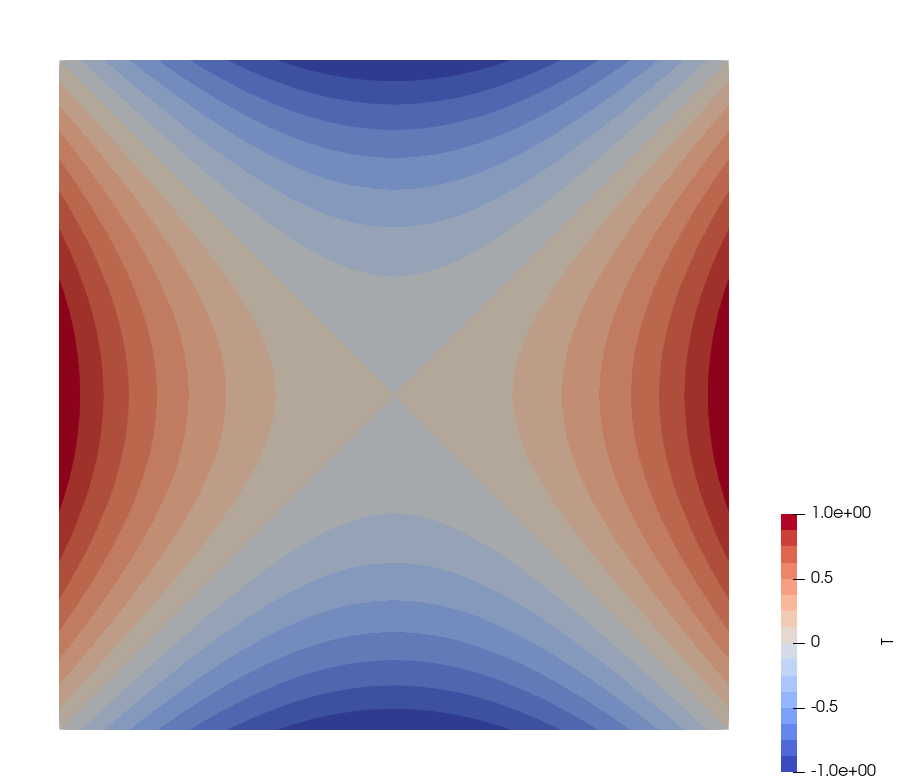
\includegraphics[height=5cm]{images/benchmark_annulus_conv/T}
\includegraphics[height=5cm]{images/benchmark_annulus_conv/arrows}\\

However, what is deeply puzzling is the fact that the temperature is exactly zero on both 
boundaries (beacuse $g(r)$ is by construction) 
and yet the temperature field is not zero in the middle, in the absence of heat source ... ?


